%!TEX output_directory = texaux
%!TEX spellcheck
%!TEX root = ../main.tex

\setlength{\abovedisplayskip}{20pt}
\setlength{\belowdisplayskip}{20pt}

\chapter{Sieci neuronowe} \label{rozdzial1}

\section{Wprowadzenie}
Sieci neuronowe to popularna w ostatnich czasach metoda uczenia maszynowego. Nazwa może słusznie przywodzi na myśl połączenia w mózgu, ponieważ właśnie one były inspiracją stojącą za powstaniem opisywanych algorytmów. Czasami używa się nazwy \textit{sztuczne sieci neuronowe}, dla wyraźnego odróżnienia ich od biologicznych odpowiedników.

Sztuczne sieci neuronowe można krótko opisać jako bardzo złożone, różniczkowalne funkcje, których parametry optymalizowane są za pomocą metod gradientowych. Żeby zastosować sieć neuronową w danym problemie, musimy spełnić dwa warunki:
\begin{itemize}
\item zdefiniować różniczkowalną funkcję kosztu;
\item zgromadzić odpowiednią ilość danych uczących, na których będziemy tę funkcję obliczać i minimalizować.
\end{itemize}

W niektórych zadaniach te wymogi mogą okazać się trudne do spełnienia. Jest to cena, którą ponosimy za uniwersalność tej metody. Ta uniwersalność sprawia, że sieci neuronowe mają zastosowanie w szerokiej gamie problemów uczenia maszynowego, od klasyfikacji \cite{imagenet}, przez kompresję obrazu \cite{compression}, aż do przetwarzania języka naturalnego \cite{rnnlm}.

Żeby ułatwić opisywanie budowy sieci neuronowej, dzieli się ją na mniejsze fragmenty nazywane warstwami. Umożliwia to składanie skomplikowanych architektur z uniwersalnych modułów. Każda warstwa sama w sobie również jest małą siecią. Możemy w uproszczeniu opisać sieć neuronową jako złożenie pewnej liczby warstw. Wektor wejściowy $x \in \mathbb{R}^n$ jest przekształcany w następujący sposób:
\[f(x) = l_L(l_{L-1}(\dots l_1(x \mid \theta_1) \dots \mid \theta_{L-1}) \mid \theta_L),\]
gdzie $L$ jest liczbą warstw, a $l_i$, parametryzowana przez zbiór $\theta_i$, funkcją obliczaną przez $i$-tą warstwę. Musi ona być różniczkowalna względem swoich parametrów. Funkcja $f$ stanowi koszt, który chcemy zminimalizować i jest zależna od $\theta = \bigcup_{i=1}^L \theta_i$.

\noindent
Wizualnie taką sieć reprezentuje ścieżka:

\begin{figure}[H]
  \centering
    \includegraphics[width=0.8\textwidth]{chapter1/img/prosta.eps}
  \caption{\small{Schemat sieci neuronowej o strukturze liniowej.}}
\end{figure}

\noindent
Jest to pewne uproszczenie, bo nic nie stoi na przeszkodzie, żeby sieć wyglądała tak:

\begin{figure}[H]
  \centering
    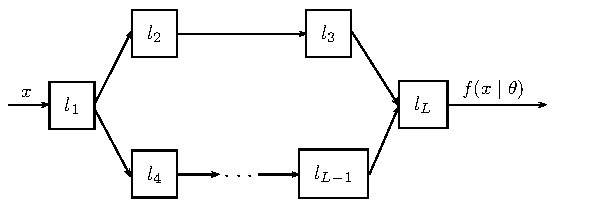
\includegraphics[width=0.9\textwidth]{chapter1/img/dag.eps}
  \caption{\small{Schemat przykładowej sieci neuronowej o strukturze DAG.}}
\end{figure}

W drugim przypadku funkcją wyliczaną przez $l_L$ może być na przykład długość konkatenacji obu wejść, albo suma elementów wyniku $l_{L-1}$ o pozycjach zadanych wynikiem $l_3$. Topologia sieci neuronowej ściśle zależy od zastosowania.

%%%%%%%%%%%%%%%%%%%%%%%%%%%%%%%%%%%%%%%%%%%%%%%%%%%%%%%%%%%%%%%%%%%%%%%%%

\section{Uczenie sieci neuronowej}
Dla uproszczenia przedstawię proces optymalizacji sieci przedstawionej na rysunku 1. Przypomnijmy, że dla punktu danych $x \in \mathbb{R}^n$ funkcja kosztu jest zadana wzorem
\[f(x) = l_L(l_{L-1}(\dots l_1(x \mid \theta_1) \dots \mid \theta_{L-1}) \mid \theta_L),\]
gdzie dla każdego $i$ $l_i$ jest funkcją parametryzowaną przez $\theta_i$, posiadającą pochodne cząstkowe względem elementów $\theta_i$. Funkcja $f$ jest zatem różniczkowalna względem elementów $\theta$. Załóżmy dodatkowo, że zbiory $\theta_1, \dots, \theta_L$ są parami rozłączne.

%%%%%%%%%%%%%%%%%%%

\subsection{Propagacja wsteczna}
Do optymalizacji $\theta$ wykorzystujemy metody gradientowe. Interesuje nas zatem obliczenie pochodnych cząstkowych $f$ względem jej parametrów.
\\\\
Wprowadźmy pomocnicze oznaczenie. Niech
\[o_i(x) = l_i(l_{i-1}(\dots l_1(x \mid \theta_1) \dots \mid \theta_{i-1}) \mid \theta_i).\]
Możemy teraz napisać
\[o_i(x) = l_i(o_{i-1}(x) \mid \theta_i)\]
oraz
\[f(x) = o_L(x).\]
\\
Przydatny będzie też fakt, że $o_i$ zależy tylko od $x$ oraz $\bigcup_{j=1}^i \theta_j$.
\\

Pochodne obliczamy korzystając z reguły łańcuchowej. Weźmy $t_L \in \theta_L$. Dla czytelności zapisu pominę argumenty funkcji. Dostajemy
\[\frac{\partial f}{\partial t_L} = \frac{\partial o_L}{\partial t_L} = \frac{\partial l_L}{\partial t_L}(o_{L-1}).\]

Ponieważ $o_{L-1}$ nie zależy od $t_L$, tutaj obliczenia się kończą. Dla przykładu weźmy teraz $t_{L-3} \in \theta_{L-3}$. Mamy
\[
\begin{aligned}
    \frac{\partial f}{\partial t_{L-3}} &= \frac{\partial o_L}{\partial t_{L-3}} = \frac{\partial l_L}{\partial o_{L-1}} \frac{\partial o_{L-1}}{\partial t_{L-3}} = \frac{\partial l_L}{\partial o_{L-1}} \frac{\partial l_{L-1}}{\partial o_{L-2}} \frac{\partial o_{L-2}}{\partial t_{L-3}} = \\[10pt]
    &= \frac{\partial l_L}{\partial o_{L-1}} \frac{\partial l_{L-1}}{\partial o_{L-2}} \frac{\partial l_{L-2}}{\partial o_{L-3}} \frac{\partial o_{L-3}}{\partial t_{L-3}}
    = \frac{\partial l_L}{\partial o_{L-1}} \frac{\partial l_{L-1}}{\partial o_{L-2}} \frac{\partial l_{L-2}}{\partial o_{L-3}} \frac{\partial l_{L-3}}{\partial t_{L-3}}(o_{L-4})
\end{aligned}
\]

W przypadku zależności kilku warstw od tego samego parametru konieczne będzie więcej aplikacji reguły łańcucha. Wzory pochodnych cząstkowych komplikują się również dla modeli o bardziej wymyślnej topologii. Ogólna zasada obliczania gradientu funkcji $f$ pozostaje jednak ta sama. W dziedzinie sieci neuronowych proces ten nosi nazwę wstecznej propagacji błędu (ang. \textit{error backpropagation}).\\

%%%%%%%%%%%%%%%%%%%

\subsection{Zbiór uczący i zbiór testowy} \label{testset}

Dotychczas mówiliśmy o funkcji kosztu zadanej na pojedynczym punkcie danych. To jednak za mało, żeby dobrać właściwe parametry. Zwykle trenowanie sieci neuronowych wymaga dużej liczby przykładów. Musimy więc zdefiniować funkcję celu $f_{tot}$ na całym zbiorze danych.

Oznaczmy zgromadzone dane przez $D$. Agregacji wartości $f$ na poszczególnych elementach $D$ często dokonuje się przez uśrednienie:
\[f_{tot}(D \mid \theta) = \frac{1}{|D|} \sum\limits_{d \in D} f(d \mid \theta)\]

Sama minimalizacja $f_{tot}$ nie wystarczy do osiągnięcia satysfakcjonujących rezultatów. Zadaniem modelu nie jest zapamiętanie danych przetwarzanych podczas uczenia, tylko bycie gotowym do pracy z nowymi przykładami. Nie wzięcie tego pod uwagę prowadzi do nadmiernego dopasowania (ang. \textit{overfitting}); model nie będzie w stanie dostarczyć przydanych wyników dla nienapotkanych wcześniej obserwacji. Jest to ogólny problem, często występujący w uczeniu maszynowym.

Istnieje wiele sposobów walki z nadmiernym dopasowaniem (inaczej \textit{regularyzacji} sieci). Mogą one polegać na przykład na zmianach w architekturze modelu lub umyślnym wprowadzaniu zaburzeń w danych. Podstawową metodą, stosowaną niemal zawsze, jest wykorzystanie zbioru testowego. Zgromadzone dane $D$ dzielimy na rozłączne podzbiory $D_{train}$ i $D_{test}$. Dokonujemy optymalizacji $f_{tot}(D_{train} \mid \theta)$. Zbiór $D_{test}$ nie jest bezpośrednio obserwowany przez model. Używamy go jedynie do sprawdzania efektywności modelu na nowych przykładach.

W sieciach neuronowych popularne jest przerywanie procesu uczenia, gdy wartość $f_{tot}(D_{test} \mid \theta)$ nie poprawia się przez zadaną liczbę $k$ kolejnych iteracji (\textit{early stopping}\label{earlys}). Pomaga to uniknąć nieproduktywnych obliczeń i nadmiernego dopasowania. Czasami, zamiast dzielić $D$ na dwa podzbiory, dokonujemy podziału na $D_{train}$, $D_{test}$ i $D_{val}$. Wówczas $D_{val}$ (tzw. zbiór walidacyjny) przejmuje rolę zbioru testowego, a z $D_{test}$ korzystamy tylko raz, dopiero po zakończeniu uczenia. W ten sposób ostateczny wynik jest obliczany w zupełnie nowym środowisku.

\begin{algorithm}[h]
    \SetAlgorithmName{Algorytm}
    \\\\podziel $D$ na rozłączne zbiory $D_{train}$, $D_{test}$, $D_{val}$\\
    $k$ -- maksymalna liczba iteracji bez poprawy\\[5pt]
    losowo zainicjuj $\theta$\\
    \While{\textnormal{była poprawa} $f_{tot}(D_{val} \mid \theta)$ \textnormal{w ostatnich} $k$ \textnormal{iteracjach}}{
        aktualizuj $\theta$ zgodnie z przyjętym algorytmem optymalizacji, korzystając z $\nabla f_{tot}(D_{train})$
    }
    ostateczny koszt to $f_{tot}(D_{test})$
    \caption{Podstawowy schemat uczenia}
\end{algorithm}

W praktyce często zdarza się, że obliczanie $\nabla f_{tot}(D_{train})$ jest bardzo kosztowne ze względu na wielkość zbioru uczącego. Z tego powodu najczęściej przed każdą iteracją losowo dzieli się $D_{train}$ na porcje (ang. \textit{batches}) stałego rozmiaru. Zamiast dokonywać jednej aktualizacji parametrów na iterację, $\theta$ jest modyfikowana po każdej porcji. Optymalizując parametry metodą gradientową traktujemy wejście $x$ jako stałą. Nadużywając oznaczenia, przez $\nabla f_{tot}$ rozumiem wektor pochodnych cząstkowych względem parametrów (nie zawierający $\partial f_{tot} / \partial x$).

\begin{algorithm}[h]
    \SetAlgorithmName{Algorytm}
    \\\\
    \While{\textnormal{była poprawa} $f_{tot}(D_{val} \mid \theta)$ \textnormal{w ostatnich} $k$ \textnormal{iteracjach}}{
        podziel $D_{train}$ na porcje $D_{train}^{(1)}, \dots , D_{train}^{(B)}$\\
        \For{$i \gets 1$ \KwTo $B$}{
            aktualizuj $\theta$ zgodnie z przyjętym algorytmem optymalizacji, korzystając z $\nabla f_{tot}(D_{train}^{(i)})$
        }
    }
    \caption{Wsadowa aktualizacja parametrów}
\end{algorithm}

%%%%%%%%%%%%%%%%%%%

\subsection{Metoda gradientu prostego}
Do minimalizacji funkcji celu względem parametrów sieci zwykle używa się jakiegoś wariantu metody gradientu prostego (ang. \textit{gradient descent}). Jest to iteracyjna metoda optymalizacji. Od punktu startowego poruszamy się w kierunku odwrotnym do gradientu. Dla wypukłej, różniczkowalnej funkcji $g(\theta)$, której pochodna spełnia warunek Lipschitza, następujący algorytm gwarantuje zbieżność do globalnego minimum:
\\[.5cm]
\begin{algorithm}[H]
    \SetAlgorithmName{Algorytm}
    \\\\zaczynamy od pewnego $\theta_0$\\
    $\alpha$ -- tempo uczenia\\[5pt]
    \For{$t \gets 1\ \KwTo\ \infty$}{
        $\theta_t \gets \theta_{t-1} - \alpha \nabla g(\theta_{t-1})$
    }
    \caption{Metoda gradientu prostego}
\end{algorithm}

\vspace{.5cm}

Zbieżność wymaga odpowiedniego doboru tempa uczenia, oraz, być może, jego modyfikacji w kolejnych iteracjach. Oprócz tego w przypadku funkcji obliczanej przez sieć neuronową teoretyczne warunki mogą nie być spełnione, a nawet najczęściej nie są. Sprawia to, że nie ma gwarancji zbieżności opisywanych metod do optymalnego rozwiązania. W praktyce jednak modyfikacje metody gradientu prostego pozwalają z powodzeniem uczyć bardzo skomplikowane sieci. Ponieważ podczas optymalizacji prawdziwej sieci aktualizacji $\theta$ dokonujemy porcjami, pełna nazwa algorytmu to \textit{stochastic gradient descent}, w skrócie \textit{SGD}.

\subsection{\textit{Adaptive Moment Estimation}} \label{adam}
Analiza wariantów \textit{SGD} nie jest tematem tej pracy, więc krótko przedstawię tylko tę wersję, z której korzystałem ucząc moje implementacje. \textit{ADAM} (\textit{adaptive moment estimation}) \cite{adam} wprowadza ważne usprawnienie do podstawowej formuły.

Pojawiają się osobne tempa uczenia dla poszczególnych elementów $\theta$. Parametr, który, ze względu na naturę danych uczących, jest wykorzystywany (a więc i aktualizowany) rzadko, teraz będzie podlegał silniejszym modyfikacjom. Z kolei taki, który pojawia się niemal wszędzie (i jest aktualizowany w prawie każdym kroku), będzie zmieniany bardzo ostrożnie. Pozwala to na większą dokładność w drugim przypadku oraz krótszy proces uczenia w pierwszym. Sprawia także, że ręczny wybór właściwego $\alpha$ przestaje być kluczowy. O tempie zmian parametru w metodzie \textit{ADAM} decydują wartości jego pierwszego i drugiego momentu, których szacowania są aktualizowane w każdym kroku.

\begin{algorithm}[h]
    \SetAlgorithmName{Algorytm}
    \\\\zaczynamy od pewnego $\theta_0$\\
    $\alpha$ -- tempo uczenia\\
    $\beta_1, \beta_2 \in [0,1)$ -- parametry aktualizacji przybliżeń momentów\\[5pt]
    $m_0 \gets 0$ -- wektor pierwszych momentów\\
    $v_0 \gets 0$ -- wektor drugich momentów\\
    \For{$t \gets 1\ \KwTo\ \infty$}{
        $g_t \gets \nabla g(\theta_{t-1})$\\
        $m_t \gets \beta_1 m_{t-1} + (1 - \beta_1) g_t$\\
        $v_t \gets \beta_2 v_{t-1} + (1 - \beta_2) g_t^2$\\
        $\hat{m}_t \gets m_t\ /\, (1 - \beta_1^t)$\\
        $\hat{v}_t \gets v_t\ /\, (1 - \beta_2^t)$\\
        $\theta_t \gets \theta_{t-1} - \alpha \hat{m}_t\ /\, (\sqrt{\hat{v}_t} + \epsilon)$
    }
    \caption{\textit{ADAM}}
\end{algorithm}
\vspace{-10pt}\small\noindent
Wszystkie operacje są nakładane na pojedyncze elementy. Górny indeks oznacza potęgowanie. Autorzy zalecają $\alpha = 10^{-3}$, $\beta_1 = 0.9$, $\beta_2 = 0.999$, $\epsilon = 10^{-8}$.\\[-10pt]
\normalsize

Warto nadmienić, że \textit{ADAM} nie wywodzi się bezpośrednio z \textit{SGD}, lecz stanowi ewolucję pomysłów i ulepszeń wprowadzonych w wielu wcześniejszych metodach, takich jak \textit{momentum} \cite{momentum}, \textit{ADAGRAD} \cite{adagrad}, \textit{ADADELTA} \cite{adadelta}, czy \textit{RMSProp} \cite{rmsprop}.

%%%%%%%%%%%%%%%%%%%%%%%%%%%%%%%%%%%%%%%%%%%%%%%%%%%%%%%%%%%%%%%%%%%%%%%%%

\section{Warstwy}
Warstwy mogą reprezentować bardzo zawiłe przekształcenia. Można jednak wyróżnić kilka najczęściej występujących typów, które stanowią podstawowy budulec większości nowoczesnych sieci. Żeby uniknąć niejasności powtórzmy, że każda warstwa sama w sobie również jest siecią neuronową. Z tego powodu często zamiast, na przykład, \textit{warstwa rekurencyjna} można przeczytać \textit{sieć rekurencyjna} w odniesieniu do tego samego obiektu.

%%%%%%%%%%%%%%%%%%%

\subsection{Warstwa afiniczna}
Najprostszą spotykaną warstwą jest warstwa afiniczna (warstwa pełna, warstwa gęsta). Jest to po prostu mnożenie przez macierz połączone z przesunięciem. Najczęściej przekształcenie kończy się nieliniowością, co pozwala na reprezentowanie skomplikowanych funkcji łącząc kilka warstw afinicznych. Przekształcenie jest zatem zadane wzorem
\[\mathit{f}(x) = \gamma(Ax + b),\]
gdzie $A \in \mathbb{R}^{m \times n}$ i $b \in \mathbb{R}^m$ są parametrami warstwy, a $\gamma$ jest nieliniowością. Notacja $\gamma(W)$ oznacza tutaj zaaplikowanie $\gamma$ do każdego elementu $W$. Taki zapis jest często spotykany w literaturze poświęconej sieciom neuronowym.
\\\\
Popularne wybory $\gamma$ to między innymi:
\begin{itemize}
\item $\gamma(z) = \mathrm{ReLU}(z) = \max(0, z)$, tzw. \textit{rectified linear unit};
\item $\gamma(z) = \sigma(z) = \frac{1}{1 + e^{-z}}$, \textit{sigmoid function};
\item $\gamma(z) = \tanh(z) = \frac{e^z - e^{-z}}{e^z + e^{-z}}$.
\end{itemize}

\vspace{5mm}
Warstwa gęsta stanowi rozwinięcie idei \textit{perceptronu} \cite{perceptron}. Perceptron oblicza znak przesuniętej, ważonej sumy elementów wejścia:
\[f(x) = \mathrm{sgn}(x^Ta + b),\]
gdzie $a \in \mathbb{R}^n$, $b \in \mathbb{R}$ są parametrem modelu, a $\mathrm{sgn}$ funkcją znaku. Może być on wykorzystywany do binarnej klasyfikacji liniowo separowalnych punktów. Pierwsza implementacja perceptronu miała miejsce w 1957 roku. Dzisiaj często służy on za przykład najprostszej sieci neuronowej.

%%%%%%%%%%%%%%%%%%%

\subsection{\textit{Softmax}}
Niektóre problemy wymagają pracy z prawdopodobieństwami. Chcąc na przykład zrobić klasyfikator o różniczkowalnym wyjściu, możemy zbudować model, który dla danego $a$ zwraca prawdopodobieństwa należenia $a$ do poszczególnych klas ze zbioru wszystkich klas $\mathbf{K} = \{1,\dots,K\}$. Wynikiem klasyfikacji jest ta klasa, której prawdopodobieństwo jest największe. W takiej sytuacji często korzysta się z funkcji \textit{softmax}, zdefiniowanej dla $z \in \mathbb{R}^{K}$ następująco:
\[(\mathrm{softmax}(z))_i = \frac{e^{z_i}}{\sum_{k \in \mathbf{K}} e^{z_k}}\]

\textit{Softmax} przekształca dowolny wektor długości $K$ w wektor liczb, które są pewnym dyskretnym rozkładem prawdopodobieństwa na wszystkie klasy. Funkcja $\exp$ funkcjonuje tutaj jako wygodna nieliniowość, dzięki której nie musimy się przejmować ujemnymi wartościami w $z$ i zyskujemy większą siłę wyrazu.

\textit{Softmax} zwykle łączy się z przekształceniem afinicznym. Pełna funkcja obliczana przez warstwę to
\[f(x) = \mathrm{softmax}(Ax + b),\]
\\
gdzie $A \in \mathbb{R}^{K \times n}$ i $b \in \mathbb{R}^{K}$ to parametry. Jest to zatem pewien szczególny przypadek wartswy gęstej, z tą różnicą, że nieliniowość nie jest nakładana na każdy element z~osobna. Dodatkowe mnożenie przez macierz pozwala nam zmienić kształt danych; wejście do funkcji \textit{softmax} musi mieć długość równą liczbie klas. W literaturze pod pojęciem \textit{softmax} może kryć się zarówno cała warstwa, jak i sama funkcja \textit{softmax}.

%%%%%%%%%%%%%%%%%%%

\subsection{Próbkowany \textit{softmax}} \label{ssoft}
\textit{Softmax}, w swojej podstawowej formie, jest mało wydajny w przypadku dużej liczby możliwych etykiet. W pracy z językiem naturalnym rolę etykiet pełnią słowa, a~tych potrafią być setki tysięcy, więc jest to dość częste zjawisko. Podczas uczenia sieci chcemy maksymalizować prawdopodobieństwo właściwej klasy $k_a \in \mathbf{K}$ dla każdego elementu $a$ w zbiorze uczącym. W przypadku klasycznego \textit{softmaxa} mamy
\[\hat{P}(k \mid a) = (\mathrm{softmax}(z))_{k} = \frac{e^{z_{k}}}{\sum_{i \in \mathbf{K}} e^{z_i}},\]
gdzie $z$ zależy od $a$. Zauważmy, że powyższe równanie można zapisać jako
\[z_k = \log(\hat{P}(k \mid a)) + C_0(a)\]
dla pewnej funkcji $C_0$ niezależnej od $k$. Oznacza to, że warstwa w sieci obliczająca $z$ tak naprawdę oblicza przesunięte logarytmy prawdopodobieństw. Oczywiście wartość przesunięcia jest nieistotna dzięki funkcji \textit{softmax}.

Do poznania wartości $\hat{P}(k_a \mid a)$ wystarczy nam tylko jeden element wynikowego wektora. Niestety, nawet do obliczenia jednego elementu musimy znać wartość $\sum_{i \in \mathbf{K}} e^{z_i}$. Przeszkodę stanowi fakt, że zwykle \textit{softmax} łączy się z warstwą afiniczną. Żeby na podstawie wektora wejściowego $x \in \mathbb{R}^n$ obliczyć mianownik \textit{softmaxa}, trzeba nałożyć na $x$ macierz $A \in \mathbb{R}^{K \times n}$, co jest dość kosztowne. Sprawia to, że w przypadku bardzo dużego $K$ zamiast pełnej funkcji \textit{softmax} stosuje się różne przybliżenia. Jednym z nich jest wersja z próbkowaniem (ang. \textit{sampled softmax}) \cite{ssoftmax}.

Opiera się ona na ograniczeniu liczby modyfikowanych parametrów w poszczególnych krokach. Będziemy rozkładać masę prawdopodobieństwa nie na całym $\mathbf{K}$, ale na jakimś mniejszym zbiorze. Pozwoli to nie wykonywać pełnego mnożenia przez macierz $A$, co z kolei spowoduje, że tylko niektóre jej wiersze będą wymagały aktualizacji.

Zaczynamy od wybrania pewnego $Q$ -- rozkładu prawdopodobieństwa na $\mathbf{K}$. Dla każdego $a$ wybieramy stałego rozmiaru próbkę $M_a$, gdzie prawdopodobieństwo wyboru $k$ wynosi $Q(k)$. Losujemy ze zwracaniem, więc $M_a$ może zawierać duplikaty. Do zgromadzonych etykiet dodawana jest właściwa, $k_a$. Nieco nadużywając notacji:
\[\hat{M}_a = M_a \cup \{k_a\}\]

Następnie należy jeszcze raz określić rozkład na $\mathbf{K}$, teraz zaopatrując model w~dodatkowy fakt: $k_a \in \hat{M}_a$. Sieć oczywiście nie wie, która klasa jest właściwa, więc jest to dla niej istotna informacja. Wie natomiast w jaki sposób powstaje zbiór $\hat{M}_a$ i może to wykorzystać obliczając koszt. Oznaczmy prawdopodobieństwo klasy $k$ dla elementu $a$ w tych nowych warunkach jako $\hat{P}(k \mid a, \hat{M}_a)$. Stosując wzór Bayesa otrzymujemy
\[\hat{P}(k \mid a, \hat{M}_a) = \frac{\hat{P}(\hat{M}_a \mid k, a)\, \hat{P}(k \mid a)}{\hat{P}(\hat{M}_a \mid a)},\]
gdzie
\[\hat{P}(\hat{M}_a \mid a) = \sum_{y \in \mathbf{K}} \hat{P}(\hat{M}_a \mid y, a)\, \hat{P}(y \mid a)\]
jest niezależne od $k$.

Zauważmy, że $\hat{P}(\hat{M}_a \mid k, a)$ to po prostu prawdopodobieństwo wylosowania zbioru $\hat{M_a} \setminus \{k\}$ ($M_a = \hat{M_a} \setminus \{k\}$ było wylosowanym zbiorem przy założeniu, że $k_a = k$). Niech dla $i \in \mathbf{K}$ $n_i$ oznacza liczbę wystąpień $i$ w $\hat{M_a}$. Wykorzystując funkcję masy rozkładu wielomianowego dostajemy
\[
\begin{aligned}
    \hat{P}(\hat{M}_a \mid k, a) &= |M_a|! \left[ \prod\limits_{i \in \mathbf{K} \setminus \{k\}} \frac{Q(i)^{n_i}}{n_i!} \right] \frac{Q(k)^{n_k-1}}{(n_k-1)!}= \\[3pt]
    & = |M_a|! \left[ \prod\limits_{i \in \mathbf{K}} \frac{Q(i)^{n_i}}{n_i!} \right]  \frac{Q(k)^{n_k-1}}{(n_k-1)!}  \frac{n_k!}{Q(k)^{n_k}} =\\[3pt]
    & = |M_a|! \left[ \prod\limits_{i \in \mathbf{K}} \frac{Q(i)^{n_i}}{n_i!} \right] \frac{n_k}{Q(k)}.
\end{aligned}
\]

\noindent
Mamy zatem
\[
\begin{aligned}
\hat{P}(k \mid a, \hat{M}_a) &= \frac{|M_a|!}{\hat{P}(\hat{M}_a \mid a)} \left[ \prod\limits_{i \in \mathbf{K}} \frac{Q(i)^{n_i}}{n_i!} \right] \frac{n_k \hat{P}(k \mid a)}{Q(k)}, \\[3pt]
\log(\hat{P}(k \mid a, \hat{M}_a)) &= C_1(a) + \log(\hat{P}(k \mid a)) - \log(Q(k)) + \log(n_k)
\end{aligned}
\]
dla pewnej funkcji $C_1$ niezależnej od $k$. Chcemy nauczyć sieć korzystać z nowej informacji, czyli obliczać
\[\hat{P}(k \mid a, \hat{M}_a) = \frac{e^{z'_{k}}}{\sum_{i \in \hat{M}_a} e^{z'_i}}.\]
Pokazaliśmy, że cel ten jest osiągnięty dla
\[
\begin{aligned}
z'_k &= \log(\hat{P}(k \mid a, \hat{M}_a)) + C_2(a) = \\[3pt]
     &= \log(\hat{P}(k \mid a)) - \log(Q(k)) + \log(n_k) + C_1(a) + C_2(a) = \\[3pt]
     &= z_k - \log(Q(k)) + \log(n_k) + C_3(a)
\end{aligned}
\]

Wartość $C_3(a)$ nie zależy od $k$, więc wystarczy do warstwy obliczającej $z_k$ dodać $- \log(Q(k)) + \log(n_k)$. W mojej implementacji z powodów wydajnościowych pomijam składnik $\log(n_k)$. W praktyce nie wydaje się to mieć negatywnego wpływu na wynik. Pozostaje dobór rozkładu $Q$. Korzystałem tutaj z częstości występowania poszczególnych słów w danych, co dało dobre rezultaty.

%%%%%%%%%%%%%%%%%%%

\subsection{Warstwa rekurencyjna} \label{rnn}
Wiele zadań sztucznej inteligencji wymaga przetwarzania sekwencji. Za przykład może posłużyć tłumaczenie maszynowe. Warstwy gęste nie radzą sobie z tym najlepiej: trzeba ograniczyć się do ciągów konkretnej długości lub przetwarzać sekwencję porcjami, poruszając się po niej oknem o stałym rozmiarze. Warstwa rekurencyjna (ang. \textit{recurrent neural network, RNN}) przetwarza elementy wejścia po kolei, aktualizując swój wewnętrzny stan. Przetwarzanie ciągu $x = (x_1, \dots, x_p), \forall_i x_i \in \mathbb{R}^n$ wygląda tak:
\[
\begin{aligned}
    & h_0 = \vv{0} \in \mathbb{R}^m \\
    & h_t = \gamma(W x_t + U h_{t-1} + b) \\
    & f(x) = h_p \in \mathbb{R}^m
\end{aligned}
\]

Wartości $W \in \mathbb{R}^{m \times n}$, $U \in \mathbb{R}^{m \times m}$, $b \in \mathbb{R}^m$ są parametrami warstwy, a $\gamma$ jest nieliniowością. Stanem początkowym $h_0$ zwykle jest wektor zerowy. W niektórych przypadkach interesują nas rezultaty częściowe. Wówczas wynikiem jest ciąg wektorów lub macierz:
\[f(x) = [h_1\ \dotsb\ h_p] \in \mathbb{R}^{m \times p}\]

Uczenie sieci rekurencyjnej polega na rozwinięciu rekurencji, a następnie konsekwentnym aplikowaniu reguły łańcucha przez całą sekwencję. Metodę tę określa się mianem wstecznej propagacji w czasie (ang. \textit{backpropagation through time, BPTT}).

%%%%%%%%%%%%%%%%%%%

\subsection{\textit{Long Short-Term Memory}} \label{lstm}
Zadaniem sieci rekurencyjnej jest modelowanie sekwencji, co czasami wiąże się z~koniecznością zapamiętywania relacji między odległymi elementami. Opisana wyżej klasyczna wersja teoretycznie jest do tego zdolna, ale optymalizacja jej za pomocą propagacji wstecznej jest bardzo trudna. Powodem jest tzw. problem znikającego gradientu (ang. \textit{vanishing gradient problem}). Wielokrotne aplikowanie reguły łańcucha sprawia, że gradient w kolejnych punktach w czasie maleje wykładniczo, często osiągając wartość bliską zeru już po kilku krokach. Powoduje to zanikanie zależności między wyrazami ciągu mocno oddalonymi w czasie \cite{hardrnn}.

\textit{Long Short-Term Memory} \cite{lstm} to zmodyfikowana wersja tradycyjnej sieci rekurencyjnej. \textit{LSTM} nie ma problemu z modelowaniem relacji pomiędzy odległymi elementami sekwencji. Kluczowym elementem tej warstwy są tzw. bramki, które decydują jak wiele informacji przenieść do kolejnego kroku rekurencji w niezmienionej formie. Pomaga to rozwiązać problem zanikających gradientów. \textit{LSTM} posiada również dodatkową pamięć, w której może przechowywać informację o wybranych wydarzeniach z przeszłości. W ten sposób ma do nich bezpośredni dostęp, więc łatwiej jej znaleźć zależności sięgające daleko wstecz.
\\
Klasyczne równania \textit{LSTM} przedstawiają się następująco:
\[
\begin{aligned}
    & c_0 = h_0 = \vv{0} \in \mathbb{R}^m \\
    & f_t = \sigma(W_f x_t + U_f h_{t-1} + b_f) \\
    & i_t = \sigma(W_i x_t + U_i h_{t-1} + b_i) \\
    & o_t = \sigma(W_o x_t + U_o h_{t-1} + b_o) \\
    & c_t = f_t \odot c_{t-1} + i_t \odot \tanh(W_c x_t + U_c h_{t-1} + b_c) \\
    & h_t = o_t \odot \tanh(c_t)
\end{aligned}
\]
\\
gdzie $b_f, b_i, b_o, b_c \in \mathbb{R}^m$, $W_f, W_i, W_o, W_c \in \mathbb{R}^{m \times n}$, $U_f, U_i, U_o, U_c \in \mathbb{R}^{m \times m}$ są parametrami przekształcenia, a $\odot$ oznacza iloczyn Hadamarda. Podobnie jak poprzednio, w zależności od zastosowania, wyjściem może być $h_p \in \mathbb{R}^m$ lub $[h_1 \dotsb h_p] \in \mathbb{R}^{m \times p}$.

Dodatkowa pamięć to wektor $c_t$. Jego aktualizacja przebiega w dwóch etapach. Najpierw następuje decyzja, które wartości pamięci należy przenieść do następnego kroku i w jakim stopniu. Odpowiada za to bramka $f_t$ (\textit{forget gate}). Następnie dodajemy do pamięci informacje o aktualnym elemencie. Bramka $i_t$ (\textit{input gate}) odpowiada za wybranie istotnych fragmentów przetworzonego wejścia. Kolejny stan, $h_t$, powstaje przez przepuszczenie pamięci przez $o_t$ (\textit{output gate}).

Eksperymenty \cite{gatesvstanh} pokazują, że \textit{LSTM} modeluje sekwencje dużo lepiej niż zwykła warstwa rekurencyjna. Dzisiaj jest to dominujący sposób implementacji rekurencji w sieci neuronowej. Wielu autorów używa pojęcia \textit{RNN}, w~rzeczywistości mając na myśli jakiś wariant \textit{LSTM}.

%%%%%%%%%%%%%%%%%%%

\subsection{\textit{Gated Recurrent Unit}}
Popularną alternatywą dla \textit{LSTM} jest zaproponowana niedawno \textit{GRU} (\textit{gated recurrent unit}) \cite{encdec}. Niesie ona ze sobą pewne uproszczenie architektury. Bramki $f_t$ i $i_t$ zostały połączone w jedną \textit{update gate}, $u_t$. Rolę zapominania informacji przejęła nowa bramka $r_t$, \textit{reset gate}. Nie ma dodatkowej pamięci. Zmiany te skutkują mniejszą liczbą parametrów i nieco niższą złożonością obliczeniową. Mimo to efektywność \textit{GRU} jest porównywalna z \textit{LSTM} \cite{gatesvstanh}.
\\
Pełna definicja warstwy:
\[
\begin{aligned}
    & h_0 = \vv{0} \in \mathbb{R}^m \\
    & u_t = \sigma(W_u x_t + U_u h_{t-1} + b_u) \\
    & r_t = \sigma(W_r x_t + U_r h_{t-1} + b_r) \\
    & \tilde{h_t} = \tanh (W x_t + U (h_{t-1} \odot r_t)  + b) \\
    & h_t = (1 - u_t) \odot h_{t-1} + u_t \odot \tilde{h_t}
\end{aligned}
\]
\\
gdzie $b_u, b_r, b \in \mathbb{R}^m$, $W_u, W_r, W \in \mathbb{R}^{m \times n}$, $U_u, U_r, U \in \mathbb{R}^{m \times m}$.

%%%%%%%%%%%%%%%%%%%

\subsection{Dwukierunkowa \textit{RNN}} \label{birnn}
Przejście po sekwencji w jednym kierunku może czasami okazać się niewystarczające. Im dłuższy ciąg, tym więcej informacji o początkowych elementach zostaje zniekształcone lub zapomniane. Czasami najnowsze elementy są najważniejsze, ale zdarza się, że ciąg stanowi zwartą całość, w której wszystkie wyrazy są bardzo istotne. Tak jest w przypadku zdań w języku naturalnym. Żeby lepiej analizować tego typu sekwencje, można skorzystać z dwukierunkowej sieci rekurencyjnej (ang. \textit{bi-directional RNN}, \textit{BRNN} lub \textit{BiRNN}).

W \textit{BiRNN} tak naprawdę mamy do czynienia z dwiema sieciami rekurencyjnymi, o osobnych zestawach parametrów. Pierwsza, $f$, przechodzi po wejściu $x = (x_1, \dots, x_p)$ tak jak zostało to opisane w sekcji~\ref{rnn}, produkując ciąg $(h_1, \dots, h_p)$. Druga, $f_r$, czyta $x$ od końca i zwraca $({h_r}_1, \dots, {h_r}_p)$:
\[
\begin{aligned}
    & f(x) = [h_1 \dotsb h_p] \in \mathbb{R}^{m \times p} \\[8pt]
    & {h_r}_0 = \vv{0} \in \mathbb{R}^{m_r} \\
    & {h_r}_t = \gamma(W_{r} x_{p-t+1} + U_r {h_r}_{t-1} + b_r) \\
    & f_r(x) = [{h_r}_1 \dotsb {h_r}_p] \in \mathbb{R}^{m_r \times p}
\end{aligned}
\]
gdzie $m_r$ jest rozmiarem stanu sieci wstecznej, a $W_r \in \mathbb{R}^{m_r \times n}$, $U_r \in \mathbb{R}^{m_r \times m_r}$, $b_r \in~\mathbb{R}^m_r$ są jej parametrami.

Następnie oba ciągi wyjściowe są agregowane do jednego wyniku. Prostym sposobem na zachowanie wszystkich informacji jest konkatenacja wektorów:
\[f_{bi}(x) =
\begin{bmatrix}
    h_1\\
    {h_r}_1
\end{bmatrix} \in \mathbb{R}^{(m + m_r)}
\]
lub też, w zależności od potrzeb:
\[f_{bi}(x) =
\begin{bmatrix}
    \begin{aligned}
        &h_1 &\dotsb \hspace{.3cm} &h_p\\
        &{h_r}_1 &\dotsb \hspace{.3cm} &{h_r}_p
    \end{aligned}
\end{bmatrix} \in \mathbb{R}^{(m + m_r) \times p}
\]
